\section{Borders Filter}

Edges are widely used in computer vision, they contain rich information about texture 
and geometry, for this reason edges are features that are usefull for several tasks, 
such as object recognition, object traking, etc.


The Sobel filter is a wellknown edge detector. To apply this filter is necessary to 
convolve the image with two 3x3 matrix, to find intensity changes in vertical and 
horizontal directions:

\begin{center}

\includegraphics[scale=0.35]{images/sobel}
\end{center}

Then both results are merged using the bellow expression and then a threshold is used to filter out non interest areas:

$$ G = \sqrt{G_x^2+ G_y^2} $$

A Sobel filter was used to obtain a representative set of points, avoiding that walls and another 
plain surfaces containing a huge amount of data, lead to an incorrect alineation.

\begin{figure}[h!]
\begin{center}
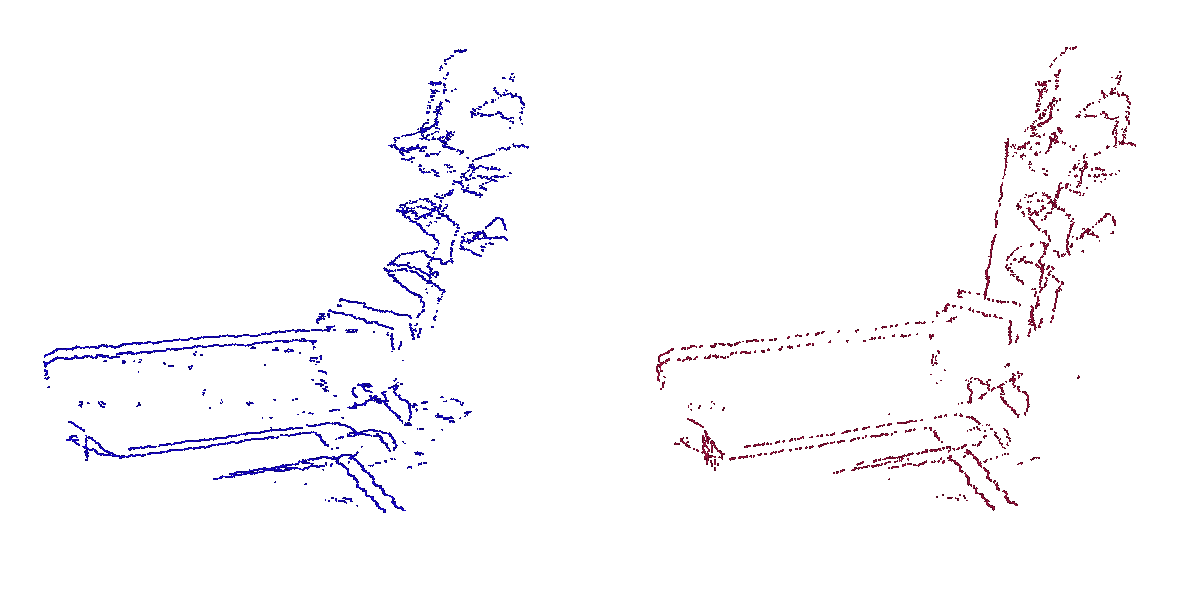
\includegraphics[scale=0.35]{images/sobel_v_h.png}
\caption{Left: Sobel vertical filtered point cloud, Right: Sobel horizontal filtered point cloud}
\end{center}

\begin{center}
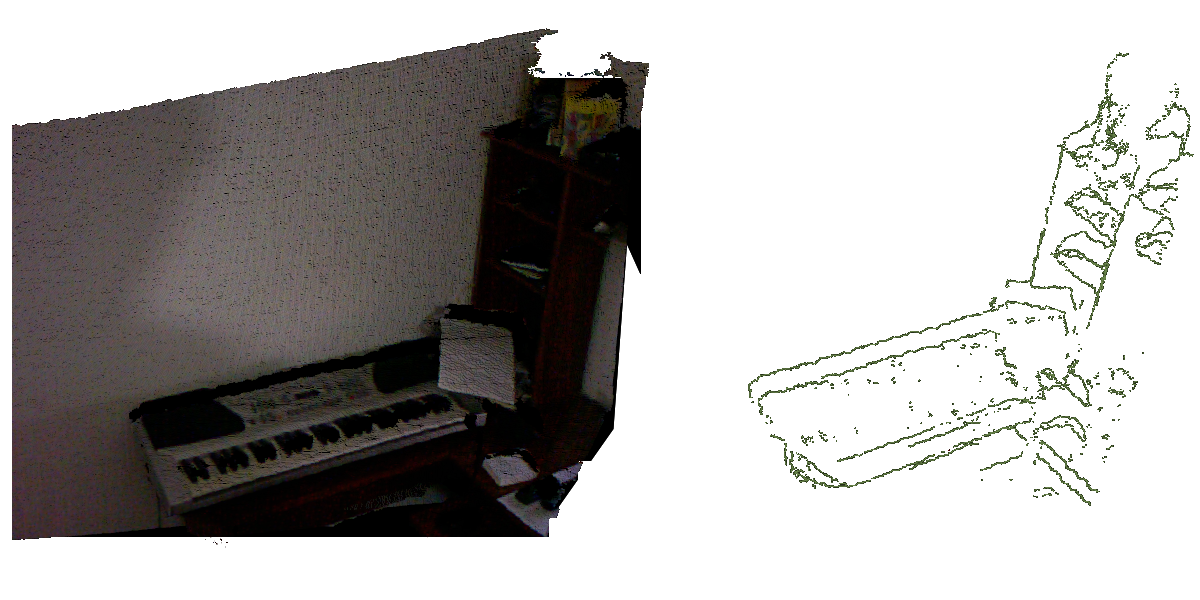
\includegraphics[scale=0.35]{images/sobel_o_g.png}
\caption{Left: Original point cloud, Right: Sobel filtered point cloud}
\end{center}
\end{figure}

There are more advanced edge filtering techniques, such as the Canny edge filter, but it involve 
a larger set of convolutions and operations. We dont need an high accuracy edge detection, the Sobel 
filter is enough to reduce the set of points used in the alineation process.
